\documentclass[a4paper,12pt]{extarticle}
\usepackage[utf8x]{inputenc}
\usepackage[T1,T2A]{fontenc}
\usepackage[russian]{babel}
\usepackage{hyperref}
\usepackage{indentfirst}
\usepackage{listings}
\usepackage{color}
\usepackage{here}
\usepackage{array}
\usepackage{multirow}
\usepackage{graphicx}
\usepackage{amsmath}
\usepackage{amssymb}
\usepackage{makeidx}    

\usepackage{caption}
\renewcommand{\lstlistingname}{Программа} % заголовок листингов кода

\bibliographystyle{ugost2008ls}

\usepackage{listings}
\lstset{ %
extendedchars=\true,
keepspaces=true,
language=C,						% choose the language of the code
basicstyle=\footnotesize,		% the size of the fonts that are used for the code
numbers=left,					% where to put the line-numbers
numberstyle=\footnotesize,		% the size of the fonts that are used for the line-numbers
stepnumber=1,					% the step between two line-numbers. If it is 1 each line will be numbered
numbersep=5pt,					% how far the line-numbers are from the code
backgroundcolor=\color{white},	% choose the background color. You must add \usepackage{color}
showspaces=false				% show spaces adding particular underscores
showstringspaces=false,			% underline spaces within strings
showtabs=false,					% show tabs within strings adding particular underscores
frame=single,           		% adds a frame around the code
tabsize=2,						% sets default tabsize to 2 spaces
captionpos=t,					% sets the caption-position to top
breaklines=true,				% sets automatic line breaking
breakatwhitespace=false,		% sets if automatic breaks should only happen at whitespace
escapeinside={\%*}{*)},			% if you want to add a comment within your code
postbreak=\raisebox{0ex}[0ex][0ex]{\ensuremath{\color{red}\hookrightarrow\space}},
texcl=true,
inputpath=source,                     % директория с листингами
}

\usepackage[left=2cm,right=2cm,
top=2cm,bottom=2cm,bindingoffset=0cm]{geometry}

%% Нумерация картинок по секциям
\usepackage{chngcntr}
\counterwithin{figure}{section}
\counterwithin{table}{section}

%%Точки нумерации заголовков
\usepackage{titlesec}
\titlelabel{\thetitle.\quad}
\usepackage[dotinlabels]{titletoc}

%% Оформления подписи рисунка
\addto\captionsrussian{\renewcommand{\figurename}{Рисунок}}
\captionsetup[figure]{labelsep = period}

%% Подпись таблицы
\DeclareCaptionFormat{hfillstart}{\hfill#1#2#3\par}
\captionsetup[table]{format=hfillstart,labelsep=newline,justification=centering,skip=-10pt,textfont=bf}

%% Путь к каталогу с рисунками
\graphicspath{{pictures/}}


\begin{document}	% начало документа

% Титульная страница
\begin{titlepage}	% начало титульной страницы

	\begin{center}		% выравнивание по центру

		\large Санкт-Петербургский Политехнический Университет Петра Великого\\
		\large Институт компьютерных наук и технологий \\
		\large Кафедра компьютерных систем и программных технологий\\[6cm]
		% название института, затем отступ 6см
		
		\huge Телекоммуникационные технологии\\[0.5cm] % название работы, затем отступ 				%0,5см
		\large Отчет по лабораторной работе №3\\[0.1cm]
		\large Линейная фильтрация
		\\[5cm]

	\end{center}


	\begin{flushright} % выравнивание по правому краю
		\begin{minipage}{0.25\textwidth} % врезка в половину ширины текста
			\begin{flushleft} % выровнять её содержимое по левому краю

				\large\textbf{Работу выполнил:}\\
				\large Балсутьев В.А.\\
				\large {Группа:} 33501/4\\
				
				\large \textbf{Преподаватель:}\\
				\large Богач Н.В.

			\end{flushleft}
		\end{minipage}
	\end{flushright}
	
	\vfill % заполнить всё доступное ниже пространство

	\begin{center}
	\large Санкт-Петербург\\
	\large \the\year % вывести дату
	\end{center} % закончить выравнивание по центру

\thispagestyle{empty} % не нумеровать страницу
\end{titlepage} % конец титульной страницы

\vfill % заполнить всё доступное ниже пространство
	

% Содержание
% Содержание
\renewcommand\contentsname{\centerline{Содержание}}
\tableofcontents
\newpage




\section{Цель работы}
Изучить воздействие ФНЧ  на тестовый сигнал с шумом.

\section{Постановка задачи}
Сгенерировать гармонический сигнал с шумом
и синтезировать ФНЧ. Получить сигнал во временной и частотной
областях до и после фильтрации. Сделать выводы о воздействии
ФНЧ на спектр сигнала.

\section{Теоретическая информация}
Линейный фильтр
\href{https://ru.wikipedia.org/wiki/%D0%9B%D0%B8%D0%BD%D0%B5%D0%B9%D0%BD%D1%8B%D0%B9_%D1%84%D0%B8%D0%BB%D1%8C%D1%82%D1%80}{(wiki)}
 — динамическая система, применяющая некий линейный оператор ко входному сигналу для выделения или 
подавления определённых частот сигнала и других функций по обработке входного сигнала.
Также довольно часто линейные фильтры называют линейные цепями(здесь и далее это синонимы).

Преобразование непрерывных сигналов в линейных цепях с постоянными параметрами может быть описано 
с помощью линейных дифференциальных уравнений с постоянными коэффициентами. Результатом интегрирования 
и дифференцирования гармонической функции некоторой частоты являются также гармонические функции той 
же частоты. Поэтому при подаче на вход линейной цепи гармонического сигнала.
$$ x(t) = A_x e^{j(2 \pi ft + \psi_x)} $$
%$$ S(\omega ) = \int_{-\infty}^{\infty} s(t)e^{-jk \omega t} dt $$
на выходе цепи будет получен гармонический сигнал, отличающийся о входного лишь амплитудой и фазой:
$$ y(t) = A_y e^{j(2 \pi ft + \psi_y)} $$
Отношение выходного сигнала цепи к входному гармоническому сигналу произвольной частоты носит название 
частотной характеристики (ЧX)$G(f)$:
$$ G(f) = \frac{y(t)}{x(t)} = \frac{A_y}{A_x}e^{i(\psi_y - \psi_x)} =  \mid G(f) \mid e^{i \psi(f)},  $$
где модуль частотной характеристики $ \mid G(f) \mid$ носит название амплитудно-частотной характеристики (АЧХ), а аргумент экспоненты  $\psi(f) $ - фазо-частотная характеристика(ФЧХ).
Если на вход цепи подается некоторое произвольное воздействие x(t), оно может быть разложено на гармонические составляющие с помощью преобразования Фурье:
$$ x(t)= \int_{-\infty}^{\infty} X(f)e^{-j \pi ft} df $$
Некоторая гармоника $х_f(t)$ частоты $f$, входящая в этот сигнал, имеет вид
$$ x_f(t) = X(f)dfe^{-j \pi ft} $$
Пройдя через линейную цепь, имеющую ЧХ $G(f)$, гармоника преобразуется в гармонику выходного сигнала:
$$ y_f(t) = x_f(t)G(f) = X(f)G(f)dfe^{-j \pi ft}, $$
из чего следует, что спектр выходного сигнала  $Y(f)$ равен произведению спектра входного сигнала цепи и ее частотной характеристики:
$$ Y(f) = X(f)G(f) $$ 
Во временной области выходной сигнал цепи $y(t)$ может быть 
найден исходя из последней формулы с помощью обратного преобразования Фурье: 
$$ y(t)= \int_{-\infty}^{\infty} Y(f)e^{-j \pi ft} df $$
Таким образом, зная ЧХ линейной цепи, можно найти описание выходного сигнала цепи вначале частотной области, а затем и во времнной.  

В данной работе будем использовать фильтр Баттерворта 
(\href{https://ru.wikipedia.org/wiki/%D0%A4%D0%B8%D0%BB%D1%8C%D1%82%D1%80_%D0%91%D0%B0%D1%82%D1%82%D0%B5%D1%80%D0%B2%D0%BE%D1%80%D1%82%D0%B0}{wiki}), для которого свойственно несколько осбенностей:
\begin{itemize}
\item АЧХ фильтра Баттерворта максимально гладкая на частотах полосы пропускания и снижается практически до нуля на частотах полосы подавления

\item Фильтр Баттерворта — единственный из фильтров, сохраняющий форму АЧХ для более высоких порядков (за исключением более крутого спада характеристики на полосе подавления) тогда как многие другие разновидности фильтров (фильтр Бесселя, фильтр Чебышёва, эллиптический фильтр) имеют различные формы АЧХ при различных порядках.

\item Амплитудно-частотная характеристика $ G(\omega ) $  фильтра Баттерворта $ n $ - го порядка может быть получена из передаточной функции $ H(s)$:

$$ G^2(\omega) = (\mid H(j \omega) \mid)^2  = \frac{G_0^2}{1 + (\frac{\omega}{\omega_c})^2n}   $$
где $n$ - порядок фильтра, $ w_c $ - частота среза(частота на которой амплитуда равна - 3 dB), $ G_0 $ - коэффициент усиления по постоянной составляющей(усиление на нулевой частоте)
\end{itemize}
 


\section{Ход выполнения работы}
Положим сигнал гармоническим и зададим его формулой 
\begin{equation}\label{eq1} 
	s(t) = \sin(2,4 \pi t)  
\end{equation}, далее прибавим к нему шумы, и получим зашумленный сигнал:
\begin{equation}\label{eq2} 
	s'(t) = \sin(2,4 \pi t) + 1,5 \cos(9 \pi t) + \frac{\sin(12 \pi t)}{2} 
\end{equation}

Чистый Сигнал и его спектр в соответствии с формулой(\ref{eq1}) принимают вид:

\begin{figure}[H]
	\begin{center}
		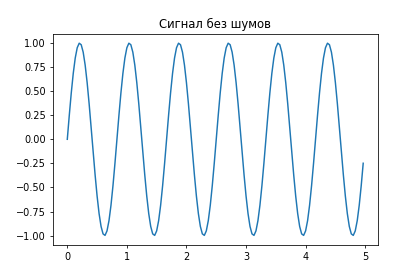
\includegraphics[scale=0.7]{001_true_sig.png}
		\caption{Чистый сигнал} 
		\label{pic:pic01} % название для ссылок внутри кода
	\end{center}
\end{figure} 
 
\begin{figure}[H]
	\begin{center}
		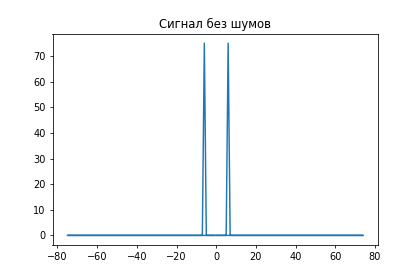
\includegraphics[scale=0.7]{002_true_sig_spec.png}
		\caption{Спектр чистого сигнал} 
		\label{pic:pic02} % название для ссылок внутри кода
	\end{center}
\end{figure} 

Реализуем вспомогательные функции для использования фильтра баттерворта и далее положим порядок фильтра $n = 6$ и частотой среза = 3,6. Выполним фильтрацию и построим отфильтрованный сигнал и зашумленный сигнал:

\begin{figure}[H]
	\begin{center}
		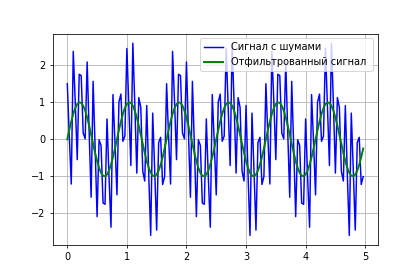
\includegraphics[scale=0.7]{003_signals.png}
		\caption{Cигналы до и после фильтрации} 
		\label{pic:pic03} % название для ссылок внутри кода
	\end{center}
\end{figure} 

Рассмотрим спектр исходного зашумленного сигнала и отфильтрованного сигнала.

\begin{figure}[H]
	\begin{center}
		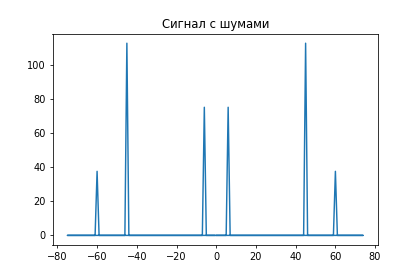
\includegraphics[scale=0.7]{004_spctr_noisy_signa.png}
		\caption{Спектр зашумленного сигнала } 
		\label{pic:pic04} % название для ссылок внутри кода
	\end{center}
\end{figure} 

\begin{figure}[H]
	\begin{center}
		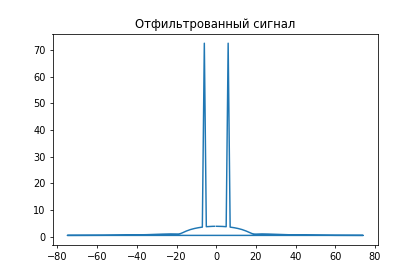
\includegraphics[scale=0.7]{005_spctr_signa.png}
		\caption{Спектр сигнала после фильтрации} 
		\label{pic:pic05} % название для ссылок внутри кода
	\end{center}
\end{figure} 


\section{Выводы}
Действительно, фильтр отметает все шумы с частотами, большими чем 1,2 и оставляет только требуемый нам сигнал(на которой наш фильтр и настроен). Так же после рассмотрения спектра чистого сигнала(\ref{pic:pic02}) и спектра сигнала после фильтрации (\ref{pic:pic05}) следует отметить
очевидную особенность - фильтр формирует не идеальный сигнал, даже несмотря на максимально гладкую АЧХ фильтра Баттерворта и 6 порядок фильтра. Но все же отличия исходного спектра следует признать пренебрежимо малыми.
  
В результате данной работы мы рассмотрели процесс линейной фильтрации с помощью фильтра Баттерворта. 
Так же нам удалось на качественном уровне разобраться с влиянием линейных фильтров на зашумленный сигнал и его спектр.


\end{document}
